\section{Evaluation}
To demonstrate the effectiveness and usefulness of our methodology, we evaluate our technique in two different scenarios: a) intra building, that is, the 
training and testing data for classification is taken from the same building, and b) inter building, where the training and testing instances are from two 
distinct buildings respectively. We also analyze how the amount of training instances and the window size of segment affect the performance of classification. We also discuss how each feature variable contributes to the classification thus helping determine when to use certain set of features. At last, we show a small application as a case study built based on the generated type information in two buildings, which would be difficult to achieve in the absence of sensor type metadata.

\subsection{Taxonomy}
In this paper, we consider 6 types of sensors, which are $CO_{2}$, humidity, room temperature, setpoint, air flow volume, other temperature. Specifically, room 
temperature includes only sensors that measure the air temperature of rooms (as ``room temp'' in Table~\ref{table:num}) and other temperature (as ``other temp'' in Table~\ref{table:num}) incorporates all other temperature measurements such as supply 
air/return air/mixed air temperature and supply/return water temperature. We also put only one general type for setpoint which includes all types of setpoints 
installed in the buildings.

\subsection{Experimental Setup}
The data we used is collected in one week from two separate buildings on two campuses. One is from the Rice Hall at 
the University of Virginia, where the sensors report to a database~\cite{trane} from every 10 seconds to every 10 minutes. The other building is the Sutardja Dai Hall (SDH) at UC Berkeley where the deployed 
sensors~\cite{keti, bacnet} report to an archiver~\cite{smap} periodically from every 5 seconds to every 10 minutes. The number of each type of sensors in 
each buidlings is given in Table~\ref{table:num} and the type ground truth for each sensor stream is expanded based on the metadata in the database.

\begin{table}[ht!]
\caption{Number of Sensors by Type}
\centering % used for centering table
\begin{tabular}{c c c}% centered columns (4 columns)
\hline %inserts single horizontal lines
Type & Rice & SDH \\ % inserts table 
\hline\hline % inserts double horizontal line
$CO_{2}$ & 16 & 52 \\ % inserting body of the table
Humidity & 48 & 52 \\
Room temp & 142 & 216 \\
Setpoint & 265 & 819 \\
Air volume & 12 & 158 \\ 
Other temp & 119 & 37 \\ \hline
Sum & 602 & 1334 \\ \hline
\end{tabular}
\label{table:num} % is used to refer this table in the text
\end{table}

All our learning and classification processes are implemented based on the scikit-learn~\cite{scikit} library, which is an open-source machine learning package implemented mostly in python and provides all the APIs in python.

\subsection{Baseline and Metrics}
As a baseline to compare our proposed approach against, we adpot a simple feature extraction scheme for each trace $F=\{med, var\}$, where $med$ and $var$ is simply the $median$ and $variance$ computed over the entire trace.

For classification, we measure the averaged cross-validation accuracy in two different scenarios (intra- and inter- buildings). In the intra-building case, the 
data from a single building is split into training and testing sets, where the results illustrate how accurate the type information can be inferred using local 
information. The inter-building experiment performs training and testing across buildings, i.e, train the classifier on the data from building A and test it 
on building B, and this set of experiments shows how much we can infer the type information of one building based on the knowledge from some other building.

For identifying potential misclassifications, we choose the true-positive rate (TPR, also known as recall), false-positive rate (FPR, also known as fall-out) and positive predictive 
value (PPV, also known as precision) as metrics to evaluate the performance of our entropy-based aprroach when making different choice of threshold. In our 
case, a true-positive (TP) is when an instance considered to be misclassified is actually a correct classification while a false-positive (FP) is when an instance 
considered to be misclassfied is misclassified.

\subsection{Classification Accuracy}
We run the two types of experiments described above, i.e, the intra- and inter- building tests, to examine the effectiveness of feature design and measure how well 
the classifier performs. We also experiment with different amount of training instances to examine how that affects the classification accuracy, which also gives 
some insight on how many instances are needed to bootstrap the classification process. The classfication results are summarized in Table~\ref{table:rice},~\ref{table:sdh},~\ref{table:rice_x},~\ref{table:sdh_x}.

\subsubsection{Intra Building Performance}
From the last column in Table~\ref{table:rice} and~\ref{table:sdh}, we see that type classification in a single building achieves accuracy of 91\% and 92\% on SDH and Rice Hall respectively, for leave-one-out (LOO) cross validation\footnote{In LOO cross validation, each learning set takes all the instances except one with the test set being the sample held out.}. The accuracy for the baseline is also shown in the table (in bracket). The only type we have difficulty differentiating is ``other temp'', which contains temperature measurements for air and water in the HVAC ventilation system, and particularly, the return air temperature measurements are almost identical to the ones mearsuring air temperature in rooms because what the return duct exhausts is mostly the air in a room.

\begin{table*}[ht!]
\centering % used for centering table
\begin{tabular}{c | c | c | c | c | c | c}% centered columns (4 columns)
\hline %inserts single horizontal lines
Type & 5\% & 10\% & 20\% & 33\% & 50\% & LOO\\ % inserts table 
%heading
\hline\hline % inserts double horizontal line
$CO_{2}$ & 51.3 (60.7) & 83.7 (94.0) & 98.4 (98.5) & 100.0 (100.0) & 93.8 (100.0) & 93.8 (100.0)\\ \hline
Humidity & 59.6 (61.8) & 66.8 (67.9) & 80.8 (77.1) & 82.3 (74.3) & 87.5 (83.8) & 83.3 (89.8)\\ \hline
Room temp & 89.0 (88.5) & 93.0 (94.0) & 95.6 (94.7) & 93.3 (95.9) & 97.2 (93.7) & 95.1 (95.6)\\ \hline
Setpoint & 97.0 (93.1) & 97.5 (95.2) & 99.2 (95.7) & 99.2 (96.5) & 98.5 (97.4) & 99.2 (97.8)\\ \hline
Air volume & 22.2 (21.8) & 35.5 (30.5) & 46.7 (49.6) & 79.2 (66.7) & 41.7 (83.3) & 83.3 (75.0)\\ \hline
Other temp & 54.7 (47.2) & 64.8 (59.0) & 70.0 (71.0) & 72.7 (75.4) & 74.7 (71.7) & 74.8 (83.1)\\ \hline
Overall & 80.4 (78.3) & 85.9 (84.4) & 90.0 (88.3) & 90.9 (90.0) & 91.4 (90.2) & 91.7 (93.3)\\ \hline
\end{tabular}
\caption{Intra-building Classification Accuracy for Rice Hall}
\label{table:rice} % is used to refer this table in the text
\end{table*}

\begin{table*}[ht!]
\centering % used for centering table
\begin{tabular}{c | c | c | c | c | c | c}% centered columns (4 columns)
\hline %inserts single horizontal lines
Type & 5\% & 10\% & 20\% & 33\% & 50\% & LOO\\ % inserts table 
%heading
\hline\hline % inserts double horizontal line
$CO_{2}$ & 80.4 (63.4) & 87.8 (75.8) & 91.4 (74.6) & 89.5 (83.7) & 92.3 (86.5) & 96.2 (76.9)\\ \hline
Humidity & 91.6 (92.4) & 94.4 (92.1) & 97.6 (95.2) & 98.1 (98.1) & 100.0 (100.0) & 98.1 (98.1)\\ \hline
Room temp & 98.3 (96.0) & 98.9 (96.3) & 99.2 (95.6) & 98.4 (94.7) & 97.7 (93.1) & 99.1 (95.8)\\ \hline
Setpoint & 99.2 (89.0) & 99.6 (90.4) & 99.5 (91.4) & 99.7 (91.8) & 99.5 (90.7) & 99.5 (93.3)\\ \hline
Air volume & 78.4 (41.8) & 87.1 (47.4) & 92.7 (52.9) & 96.8 (57.1) & 98.7 (55.3) & 97.5 (57.1)\\ \hline
Other temp & 23.7 (19.4) & 38.4 (28.7) & 62.3 (36.5) & 68.9 (48.7) & 75.7 (59.9) & 73.0 (59.5)\\ \hline
Overall & 93.4 (81.4) & 95.6 (83.7) & 97.2 (85.2) & 97.8 (86.6) & 98.2 (86.0) & 98.3 (87.7)\\ \hline
\end{tabular}
\caption{Intra-building Classification Accuracy for SDH}
\label{table:sdh} % is used to refer this table in the text
\end{table*}

\subsubsection{Inter Building Performance}
This set of experiments illustrates how accurately we can refer the type information of one building based on the knowledge from another building. The overall accuracy for the two buildings by training on the entire data set (train on SDH for Rice and train on Rice for SDH) is around 82\%, as seen from the last columns in Table~\ref{table:rice_x} and~\ref{table:sdh_x}. Particularly, we see that the accuracy for ``other temperature'' in Rice is abnormal compared to the rest of the
results. The issue with classifying ``other temperature'' in Rice is that there are many traces measuring the temperatrue of supply and return cold/hot water circulated in the ventilation system, which are abscent in the Berkeley building as a training set. Therefore the feature of these traces cannot be learned from SDH, which causes problem to classifying these traces.

\begin{table*}[ht!]
\centering % used for centering table
\begin{tabular}{c | c | c | c | c | c | c}% centered columns (4 columns)
\hline %inserts single horizontal lines
Type & 5\% & 10\% & 20\% & 33\% & 50\% & 100\% \\ % inserts table 
%heading
\hline\hline % inserts double horizontal line
$CO_{2}$ & 29.7 (44.4) & 45.6 (56.9) & 75.0 (75.0) & 93.8 (72.9) & 93.8 (75.0) & 87.5 (93.8)\\ \hline
Humidity & 50.9 (30.5) & 72.1 (26.7) & 76.2 (28.6) & 76.4 (21.1) & 89.6 (16.3) & 87.5 (26.5)\\ \hline
Room temp & 97.6 (92.7) & 99.4 (91.4) & 100.0 (90.9) & 97.2 (92.5) & 100.0 (93.1) & 100.0 (91.8)\\ \hline
Setpoint & 97.8 (94.7) & 98.2 (94.6) & 98.0 (92.8) & 97.7 (91.4) & 97.5 (92.3) & 98.9 (92.6)\\ \hline
Air volume & 57.5 (21.2) & 58.3 (18.3) & 66.7 (23.3) & 63.9 (25.0) & 70.8 (20.8) & 83.3 (25.0)\\ \hline
Other temp & 5.3 (5.8) & 10.8 (6.2) & 11.1 (6.9) & 16.8 (10.2) & 18.9 (10.5) & 19.3 (12.9)\\ \hline
Overall & 73.1 (69.1) & 76.9 (68.7) & 78.3 (68.7) & 79.1 (68.5) & 81.3 (68.7) & 81.9 (70.3)\\ \hline
\end{tabular}
\caption{Inter-building Classification Accuracy for Rice Hall}
\label{table:rice_x} % is used to refer this table in the text
\end{table*}

\begin{table*}[ht!]
\centering % used for centering table
\begin{tabular}{c | c | c | c | c | c | c} \hline
Type & 5\% & 10\% & 20\% & 33\% & 50\% & 100\%\\ % inserts table 
\hline\hline % inserts double horizontal line
$CO_{2}$ & 63.5 (94.2) & 96.9 (96.2) & 90.8 (96.9) & 93.6 (94.9) & 92.3 (95.2) & 98.1 (98.1)\\ \hline
Humidity & 67.4 (28.8) & 86.3 (47.4) & 98.1 (45.0) & 96.2 (41.0) & 98.1 (25) & 98.1 (44.2)\\ \hline
Room temp & 78.0 (78.0) & 78.2 (75.8) & 72.9 (73.8) & 77.9 (76.7) & 80.3 (77.3) & 53.2 (77.3)\\ \hline
Setpoint & 77.4 (53.3) & 83.3 (50.8) & 86.5 (53.4) & 87.9 (54.4) & 87.2 (62.0) & 91.8 (58.1)\\ \hline
Air volume & 13.8 (34.7) & 15.2 (33.1) & 37.8 (25.1) & 42.4 (32.9) & 50.3 (30.3) & 71.5 (38.8)\\ \hline
Other temp & 48.3 (51.4) & 49.7 (53.1) & 58.4 (4.6) & 45.0 (52.3) & 45.9 (54.1) & 67.6 (51.4)\\ \hline
Overall & 68.2 (55.5) & 74.1 (54.3) & 78.4 (54.5) & 80.3 (56.2) & 81.2 (60.1) & 83.0 (59.6)\\ \hline
\end{tabular}
\caption{Inter-building Classification Accuracy for SDH}
\caption*{Each table shows the averaged classification accuracy (in the last column only for intra-building case) and the accuracy of experiments where different percentage of the complete training set is used (denoted as `X\%'). In the percentage analysis, each percentage is repeated 1/percent times and the averaged accuracy is calculated as presented in the tables.}
\label{table:sdh_x} % is used to refer this table in the text
\end{table*}

\subsection{Learning Bootstrapping}
In Table~\ref{table:rice},~\ref{table:sdh},~\ref{table:rice_x},~\ref{table:sdh_x}, the last columns demonstrate how accurately we can do classification on average. There also remains the question of how many number of instances we need to bootstrap the learning process for both of the intra- and inter- building cases. To examine the impact of number of instances on classification accuracy, we use different percentage of the original data set as training set, i.e, 5\%, 10\%, 20\%, 33\%,
50\%, and the results are presented as the first five columns in each table. For each percentage of training process, we apply stratified sampling\footnote{The sampled set contains the same percentage of samples of each class as the original complete set.} on the original set and repeat the same percentage 1/percentage times to get an averaged accuracy for that percentage. We can clearly see a trend that more
training instances yield better classification results in all cases. However, we can also notice that after having 20\% of the complete set (which is $\sim$120 instances and $\sim$260 instances for Rice and SDH respectively) the accuracy doesn't increase too much even reaching 50\% of the complete set. This indicates that we don't need too many instances to bootstrap the learning process within or across buildings to accomplish sensor type classification tasks.

\subsection{Window Size Sensitivity}
Remember that all the above classification results were obtained using features extracted in 45-minute long window on the original sensor traces. To corroborate our decision, we study how different size of time window affects the classification and Figure~\ref{fig:window} shows the results. Intra- case performs LOO cross validation while inter- case runs 10-fold cross validation. For intra-building case, the classification is not sensitive to different window size as can be seen in the figure: basically, accuracy stays almost the same for both buildings because within the same building, as long as we can capture the short term characteristics in windowed time slots for sensor dynamics, the size of the time window doesn't make much difference. However, for the inter-building case, the time window size matters in the way that the local micro-climate in one building can be quite different from another, we need to ``tune'' this common short term window to capature the dynamics that can be used to infer type information across buildings. Therefore, even though we achieve decent type classification accuracy across buildings, (i.e, use information from one building to help classify the traces in another building), we still need to optimize the size of time window, which is 45 minutes in our case. We believe this ``tuning'' is significant to such kind of learning across buildings and is straightforward to achieve in general.

\begin{figure}[ht!]
\centering
	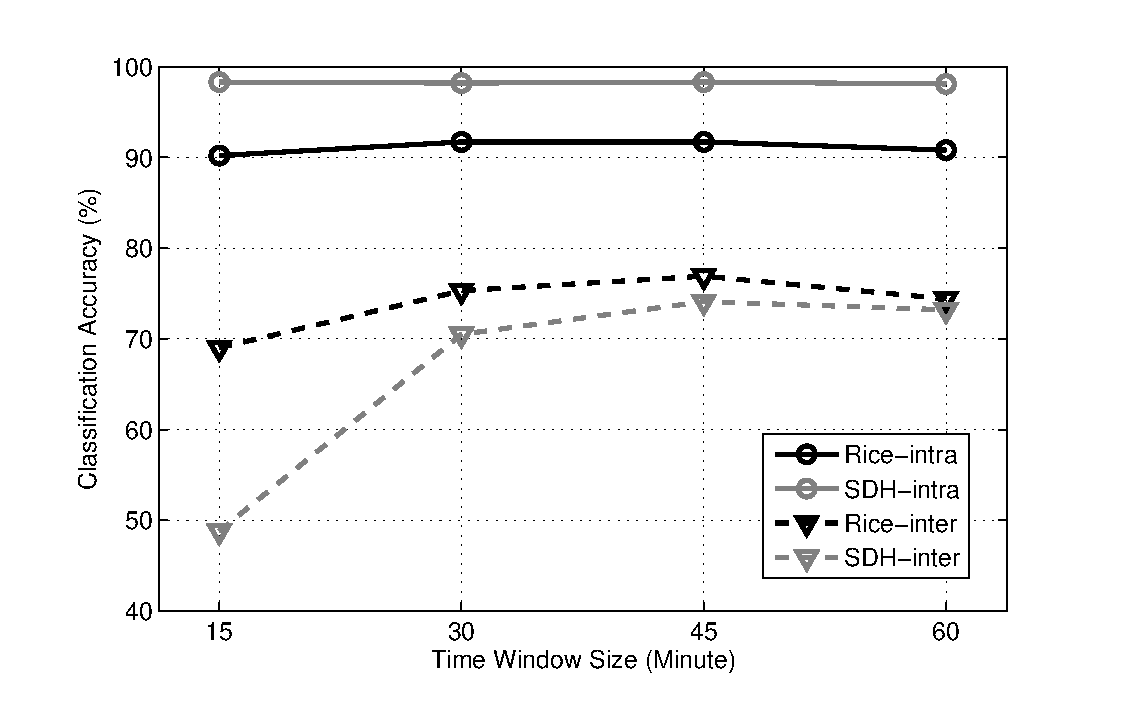
\includegraphics[width=0.45\textwidth]{./fig/window.eps}
\caption{Classification accuracy for intra- and inter- building against different size of time window. A window size of 45 minutes is optimal for our classification tasks.}
\label{fig:window}
\end{figure}

%\subsection{Feature Importance and Selection}
\subsection{Identifying Potential Misclassification}
As we discussed in early section, being able to identify misclassified instances in sensor type classification is vital to improving the overall accuracy. To identify potential misclassified instances, we propose to quantify the ``uncertainty'' of classification with the entropy-based approach described in Section 3.3. Figure~\ref{fig:cdf} shows the CDF of class probability entropy of classification in the intra- and inter- building scenarios. We see that the collection of correct
classification (solid lines) has a distinct distribution from the collection of misclassfication (dotted lines). Based on such distinction in the distribution, we can choose a certain entropy value as threshold and filter out all the classified instances whose class probablity entropy is greater than the threshold outputted by the forest. Figure~\ref{fig:roc} illustrates the performance of our entropy-based approach to identifying potential misclassification. Here are the definitions needed to understand the statistics:

$S_{1}$: the set of instance whose class probablity entropy is greater than the threshold.

$S_{2}$: the set of instance falling in $S_{1}$ that is misclassified in the classfication process.

$S_{3}$: the set of instance falling in $S_{1}$ that is correctly classified in the classfication process.

$S_{4}$: the set of instance that is misclassified in the classfication process.

$S_{5}$: the set of instance that is correctly classified in the classfication process.

And, 
\begin{displaymath}
TPR = \frac{|S_{2}|}{|S_{4}|},\quad
FPR = \frac{|S_{3}|}{|S_{5}|},\quad
PPV = \frac{|S_{2}|}{|S_{1}|},\quad
\end{displaymath}
Where $|\cdot|$ is the cardinality of a set. We see that as the threshold value increases, both the TPR (recall) and FPR (fall-out) decrease while the PPV (precision) keeps increasing. In our case, a smaller threshold essentially leads to more instances being filtered out as potential misclassification ``candidates'' thus helping identify more acutal misclassified instances. However, the more candidates we filter our, the more instances we need to manually inspect,
which inevitably leads to lower precision of the identificatoin process. So we want to strike a balance between achieving a high recall rate as well as maintaining a high precision. As a result, we suggest picking a threshold somewhere between 0.4 and 0.45 is appropriate. In intra-building case, such a threshold (0.4~0.45) helps identify $\sim$30\% of the misclassified instances for Rice and $\sim$50\% for SDH while resulting in that $\sim$70\% and $\sim$50\% of the instances
needing manual inspection are correct classification, for Rice and SDH respectively. As for the inter-building case, our approach is able to identify $\sim$75\% of the misclassified instances for both Rice and SDH with an overhead of $\sim$40\% and $\sim$70\% in the inspection candidates, for Rice and SDH respectively.

\begin{figure*}[ht!]
\centering
	\begin{subfigure}{0.48\textwidth}
                \centering
		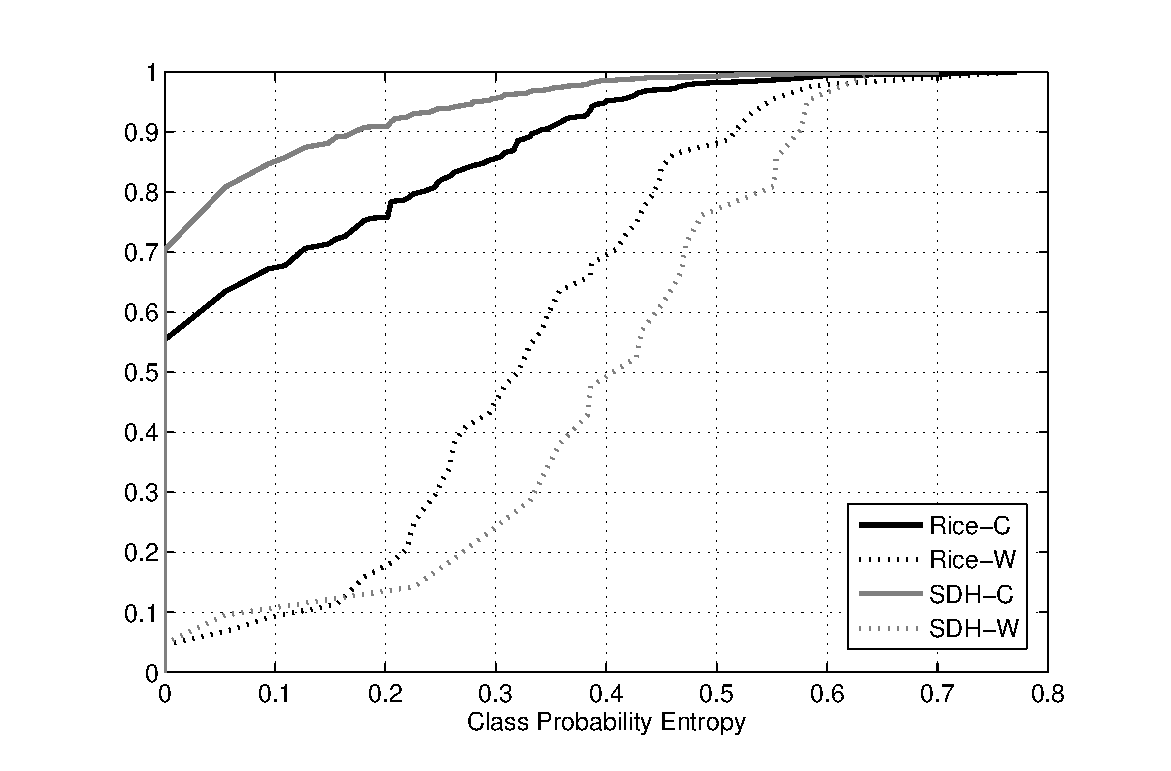
\includegraphics[width=\textwidth]{./fig/cdf_intra.eps}
                \caption{Intra-building Classification}
                \label{fig:cdf_intra}
	\end{subfigure}
	\begin{subfigure}{0.48\textwidth}
                \centering
		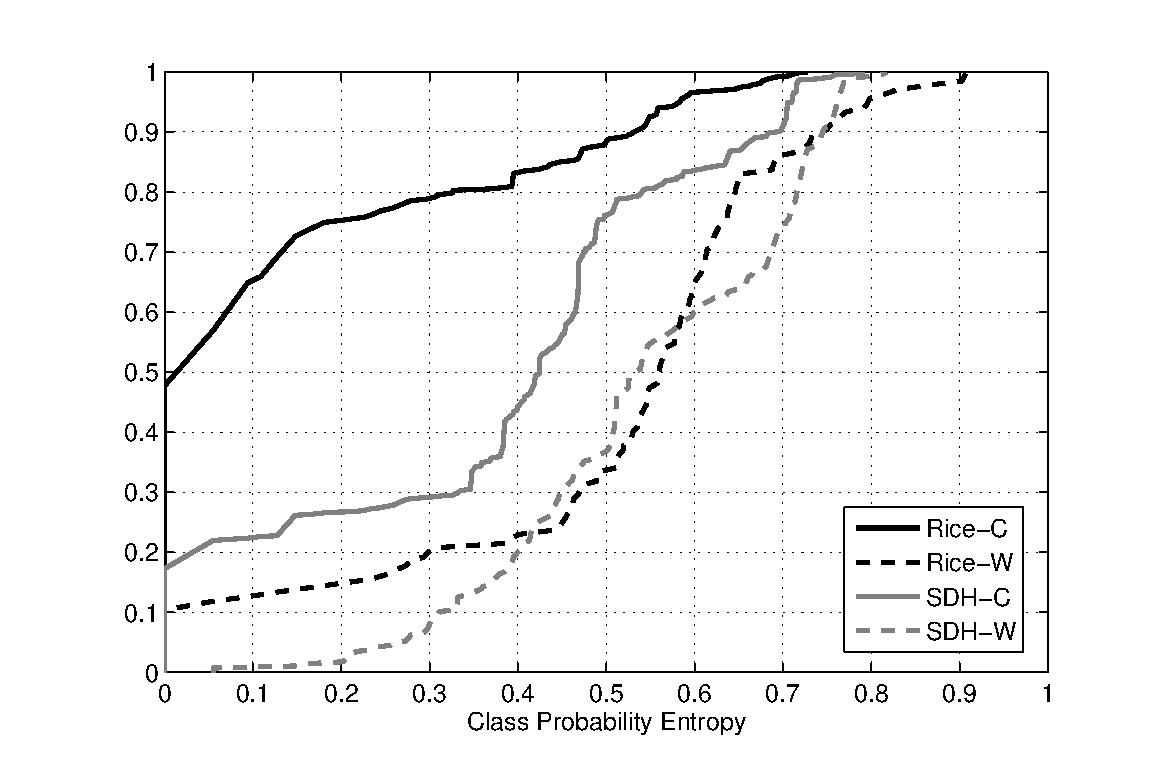
\includegraphics[width=\textwidth]{./fig/cdf_inter.eps}
                \caption{Inter-building Classification}
                \label{fig:cdf_inter}
	\end{subfigure}
\caption{The CDF curves depict the class probability entropy distribution for the both collection of correct and wrong classification in the intra- and inter- building test cases.}
\label{fig:cdf}
\end{figure*}

\begin{figure*}[ht!]
\centering
	\begin{subfigure}{0.48\textwidth}
                \centering
		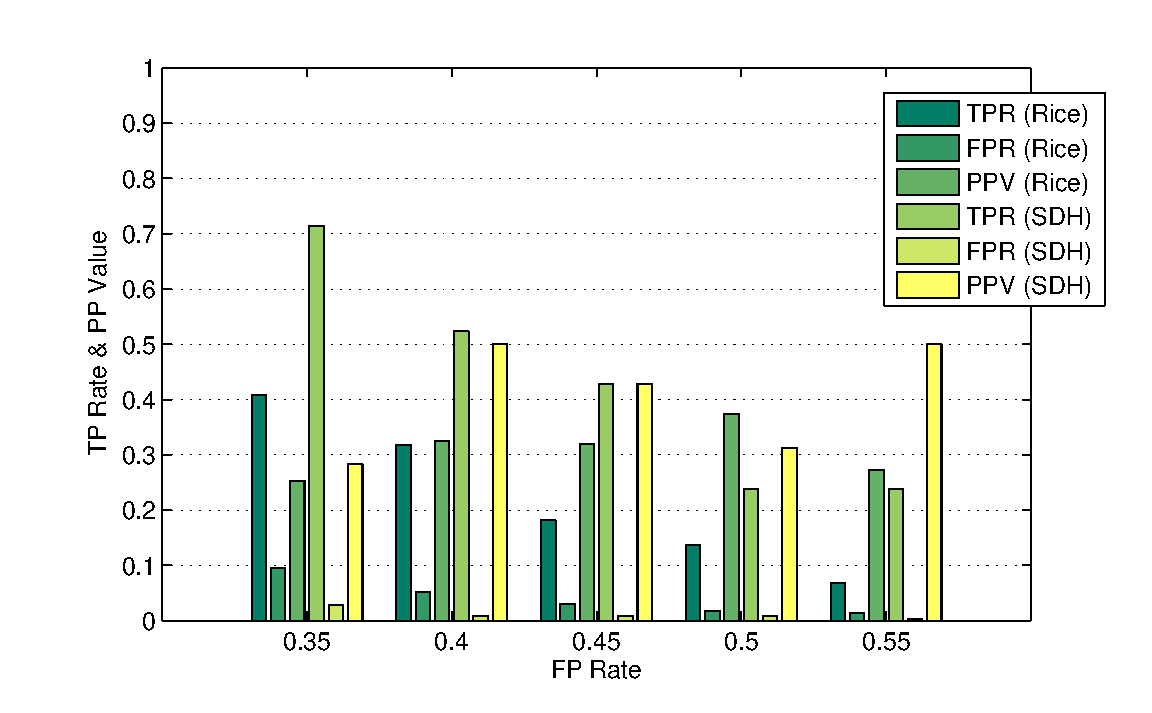
\includegraphics[width=\textwidth]{./fig/roc_intra.eps}
                \caption{Intra-building Performance}
                \label{fig:roc_intra}
	\end{subfigure}
	\begin{subfigure}{0.48\textwidth}
                \centering
		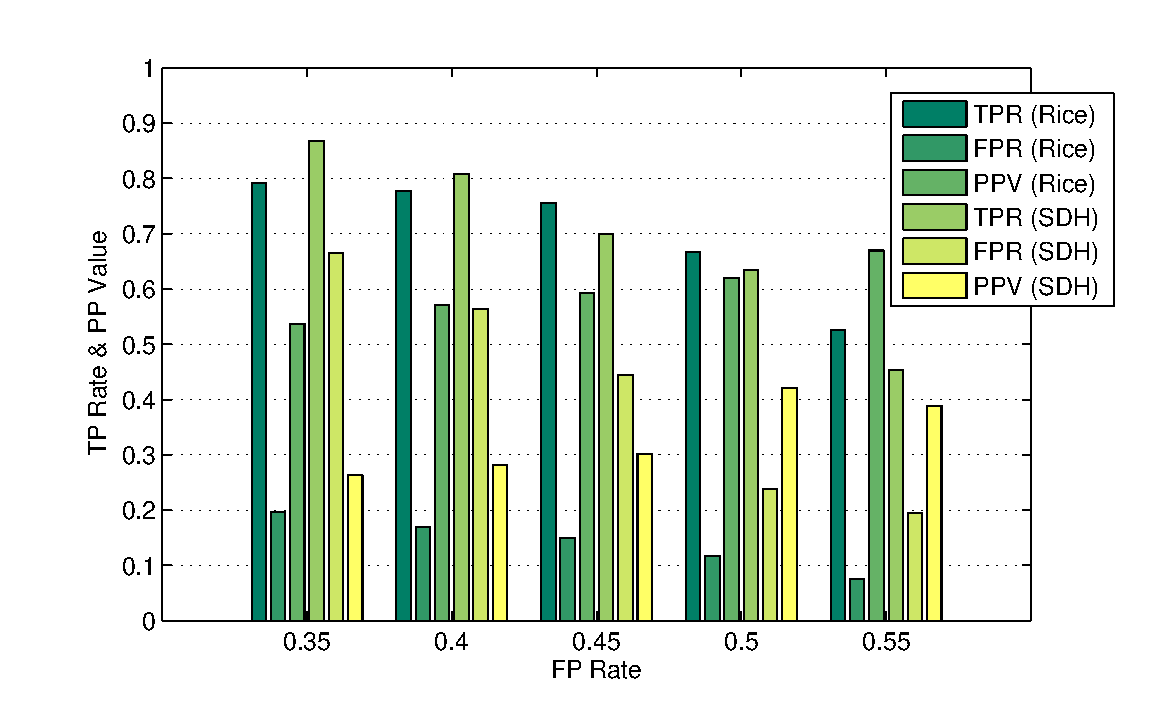
\includegraphics[width=\textwidth]{./fig/roc_inter.eps}
                \caption{Inter-building Performance}
                \label{fig:roc_inter}
	\end{subfigure}
\caption{The ROC curves depict the sensitivity of misclassification identification to different entropy threshold value. Choosing a threshold somewhere between 0.4 and 0.45 achieves the best compromise between recall and precision. }
\label{fig:roc}
\end{figure*}

%\subsection{Case Study}
%TBD
